\chapter{Planification}

\section{Hiérarchie des tâches}
Les différentes tâches de notre projet sont regroupée dans le tableau suivant \ref{fig::taches}. Nous n'avons représenté ici que les tâches englobantes pour une meilleure lisibilité. On retiendra notamment la partie construction encore divisée en trois parties comme le montre la figure \ref{fig::chrono}.

Notre projet arrive ici à environ 730 heures de travail, ce qui est ce que nous avions prévu. Nous avons été généreux sur la durée des tâches au second semestre, car le changement d'effectif risque d'affecter la progression du projet.

\begin{figure}[H]
	\centering
	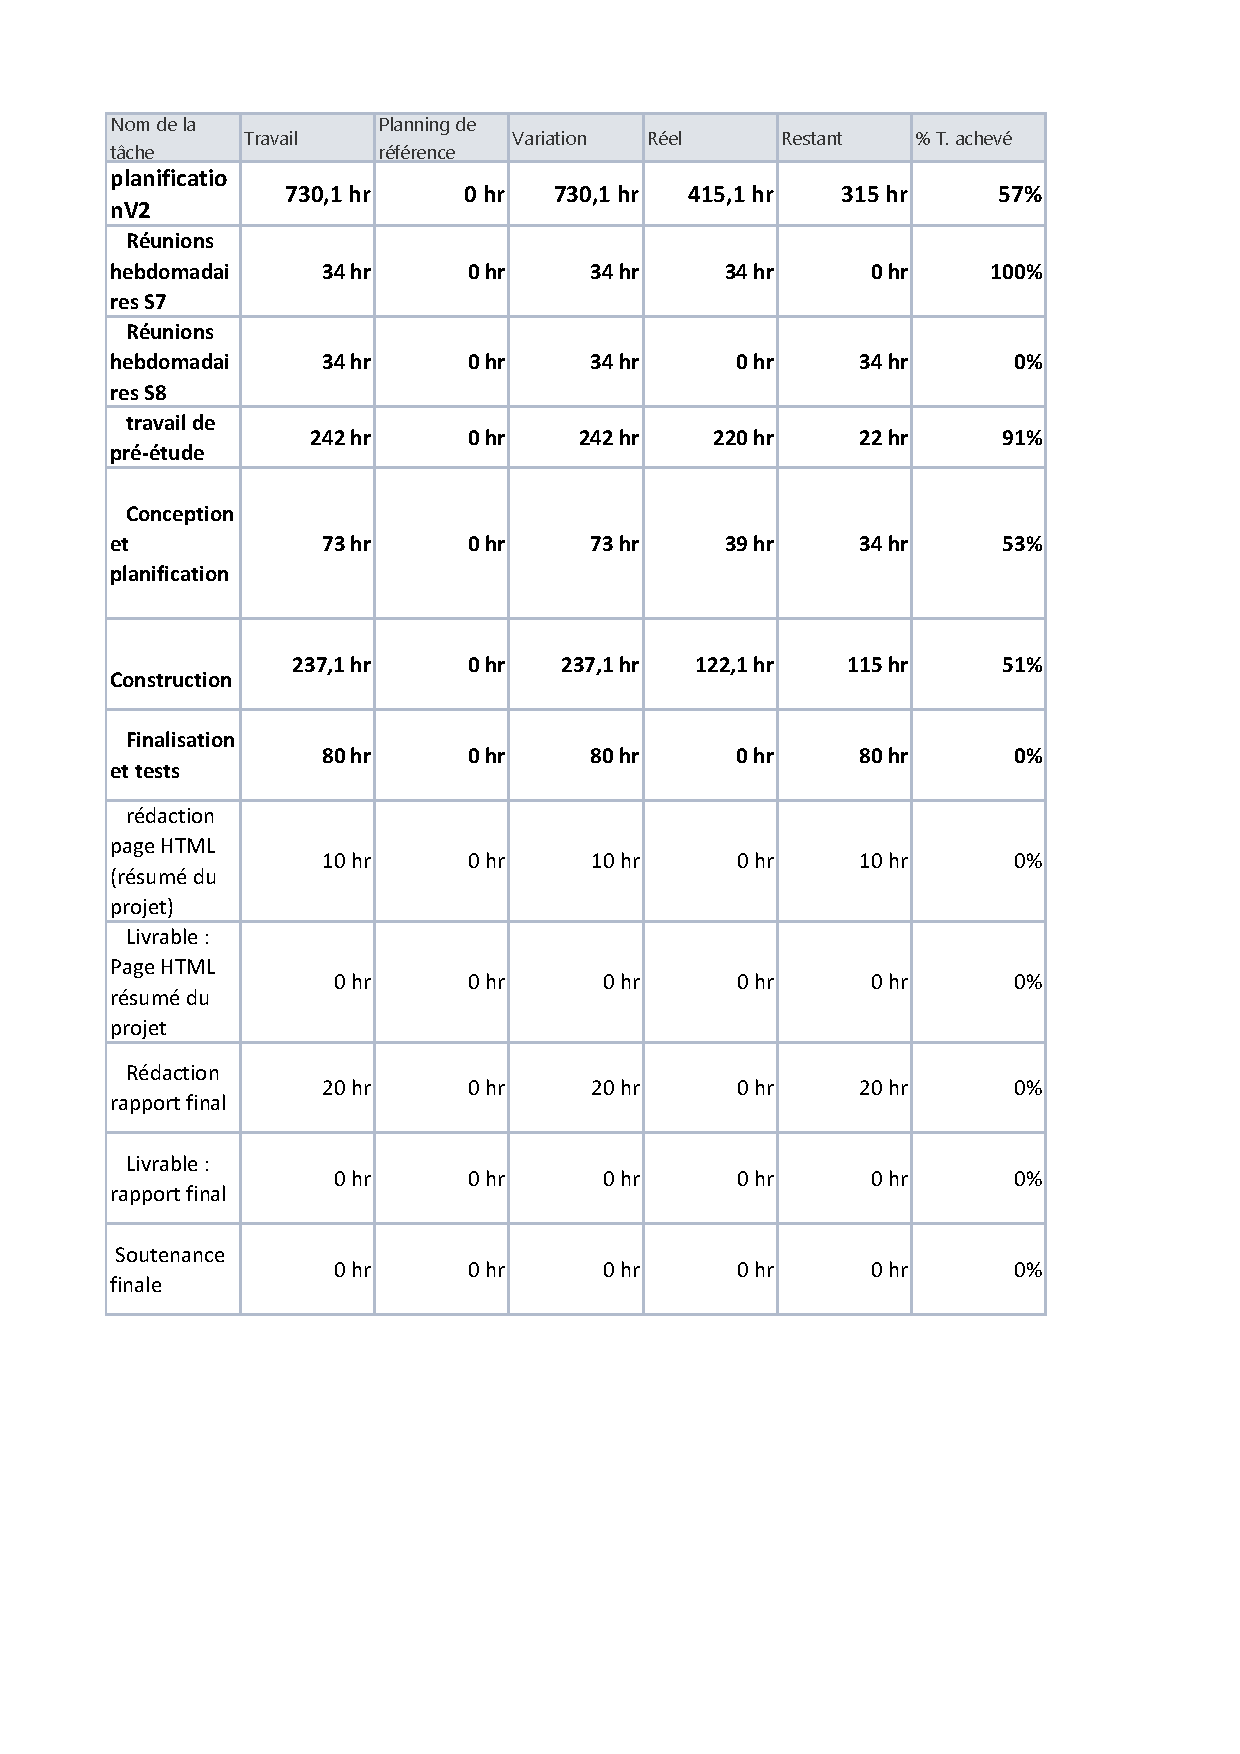
\includegraphics[scale=0.5]{images/taches.pdf}
	\caption{Tableau des tâches}
	\label{fig::taches}
\end{figure}

\section{Affectation des ressources}
Nous avons décidés, après concertation, que nous serions capables de travailler en moyenne une heure par jour sur le projet. Nous avons aussi défini certaines périodes de congés, correspondant plus précisément à nos semaines de partiels, ainsi que les vacances où nous consacreront en moyenne une heure et demi au projet. Avec cela, nous avons obtenus le tableau d'affectation des ressources suivant \ref{fig::ressources}. Nous avons décidé de garder cette capacité de travail car elle se base sur la réalité. Nous obtenons donc une répartition de travail assez légère. Nous serons par conséquent capables de disposer de beaucoup de temps pour corriger des bugs dans l'application. Ceci s'avèrera crucial car l'application doit servir tout au long de l'année pour gérer les mobilité du département informatique.

Au second semestre, la capacité maximale a été réduite à 300  (700 au premier semestre) ce qui explique une charge moins importante.

\begin{figure}[H]
	\centering
	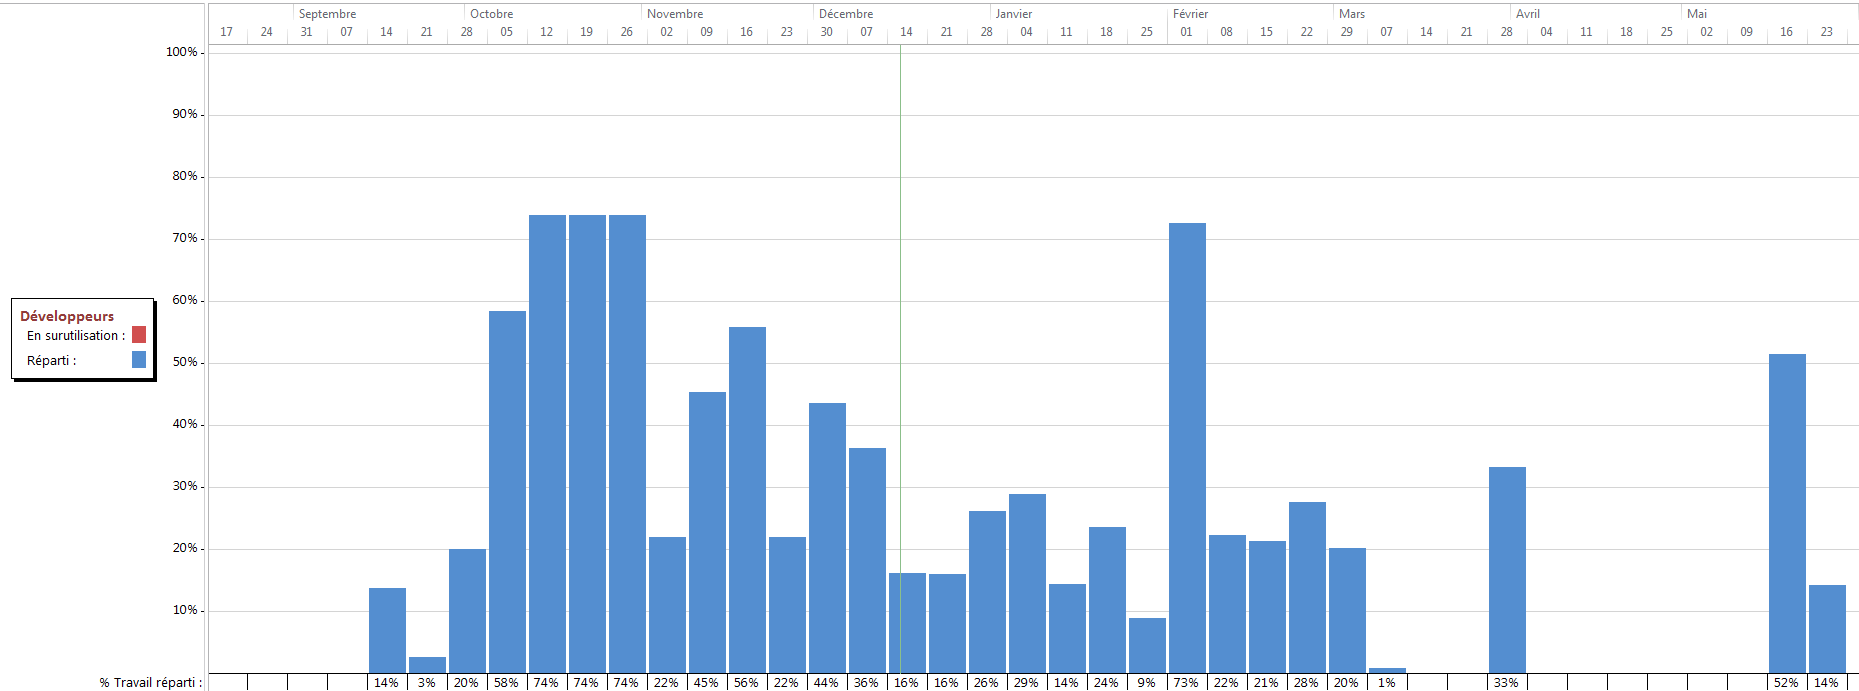
\includegraphics[angle=90,scale=0.35]{images/ressources.PNG}
	\caption{Tableau des ressources}
	\label{fig::ressources}
\end{figure}

\section{Planning}
\begin{figure}[H]
	\centering
	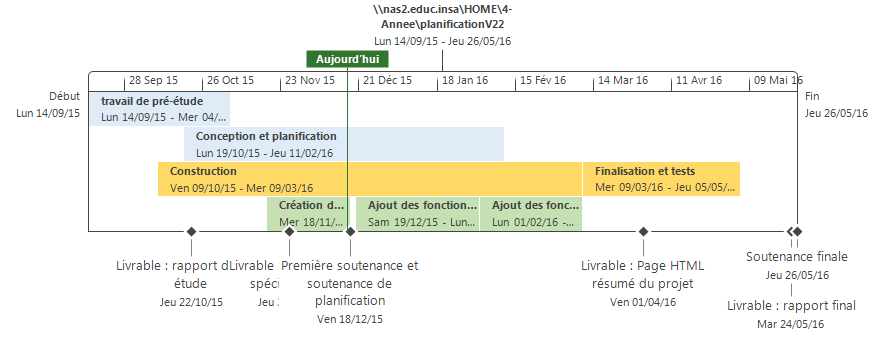
\includegraphics[scale=0.7]{images/chrono_planif.png}
	\caption{Chronologie du projet}
	\label{fig::chrono}
\end{figure}

Notre planning restera étroitement lié aux différentes étapes du suivi des mobilités. La construction de l'application se fera donc en trois étapes (en vert sur le schéma \ref{fig::chrono}) :
\begin{itemize}
 \item la création d'un prototype proposant les fonctionnalités nécessaires à la première étape (vœux et affectations).
 \item la gestion des fichiers nécessaires à la mobilité (dépôt sur le site, et apposition électronique de la signature).
 \item le suivi des étudiants à l'étranger.
\end{itemize}
Nous travailleront donc de façon itérative, en proposant une application fonctionnelle, un peu plus complète à la fin de chaque étape. Nous vérifieront le bon fonctionnement avec des tests sur les mobilités de cette année au département INFO, avant de délivrer une nouvelle version. 


Suite à cela, nous avons réservé beaucoup de temps à la finalisation du projet. Celui-ci étant destiné à devenir une application pérenne, au service de l'INSA de Rennes, il est nécessaire de s'assurer de sa stabilité. Nous travailleront aussi le design du site durant cette étape. 

\begin{figure}[H]
	\centering
	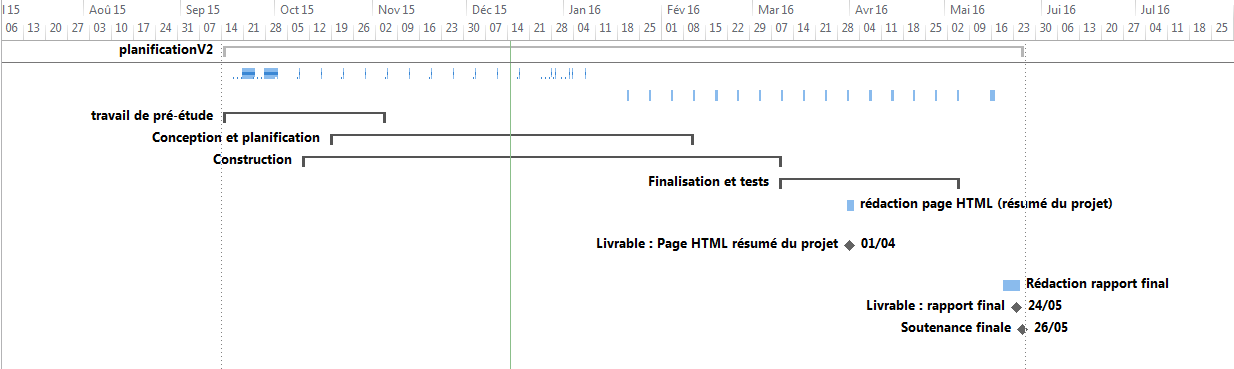
\includegraphics[scale=0.5]{images/gant.PNG}
	\caption{GANT (réduit aux grandes parties du projet)}
\end{figure}

